\chapter{Problem Context and Related Work}

%\chapter*{Introducere}
\label{intro}

\tolerance=9999
\emergencystretch=3em

\indent \par This chapter sets the stage for the rest of the thesis. It starts with the problem itself: why delivering on-demand audio from the cloud has become expensive, and why the egress bandwidth bill is the part worth attacking first. It then breaks peer-assisted streaming into the handful of design domains that any such system has to handle, surveys the candidate solutions for each one, and reviews the older systems that combined them. The aim here is deliberately limited to mapping the design space and weighing the trade-offs, as the quantitative argument that turns those trade-offs into one committed design is the work of Chapter \ref{chap:ch2}.

\section{Problem Context}

\indent \par On-demand multimedia streaming has changed the way people consume music and video, but it has also made delivery costs harder to ignore. Most streaming platforms still depend on centralised cloud infrastructure and CDNs (Content Delivery Networks). Every request to listen to a song creates a small bandwidth fee for the provider, usually called egress, and that small fee grows into a serious bill when the user base grows. This cost model is not hidden in fine print: AWS, Google Cloud and Azure all expose public data-transfer-out pricing pages, treating bytes leaving the cloud as a first-class billable resource \cite{aws_global_network_faq,google_cloud_network_pricing,azure_bandwidth_pricing}.

\par For a while, this problem was manageable. The rapid growth of AI workloads has changed the industry quickly, and cloud capacity has become a harder financial problem for companies that already move a lot of data. Modern streaming services use machine learning for real-time recommendation, user sentiment analysis, adaptive bitrate optimisation and predictive analytics. These systems improve the user experience, but they also compete for the same cloud resources and push operating costs upward.

\par Back in 2018, Spotify signed a deal with Google to spend a minimum of \$447 million on the Google Cloud Platform during the first three years of service \cite{spotify_google}. Over the same period shown in Figure \ref{fig:spotify_economics_indexed}, Spotify Premium moved from \$9.99 in 2018 to \$12.99 in 2025 \cite{spotify_prices}, after several consecutive increases. The reasons are not limited to bandwidth, of course, but rising operating costs, pandemic-era inflation and AI workloads competing for the same cloud capacity all squeeze provider margins and are eventually felt by the end consumer. The egress bandwidth targeted in this thesis has a cleaner shape: it is billed per gigabyte and scales with the number of listeners, regardless of those wider price movements. That is what makes it worth attacking directly. If streaming is to stay economically reasonable, the delivery path has to become cheaper for the provider without becoming worse for the listener.

\par The irony is that peer-assisted delivery is not foreign to music streaming. Before its full cloud migration, Spotify itself used a low-latency P2P music-on-demand architecture, measured by Kreitz and Niemel\"a as a large-scale production system \cite{spotify_p2p}. Later work on integrating smartphones into the same peer-assisted model showed why mobile devices cannot simply be treated as desktop peers, especially when battery state and radio access change during the day \cite{spotify_mobile_p2p}. The goal here is therefore not to reinvent generic file sharing, but to recover the useful part of that older architecture under modern browser, mobile and cloud constraints.

\begin{figure}[htbp]
    \centering
    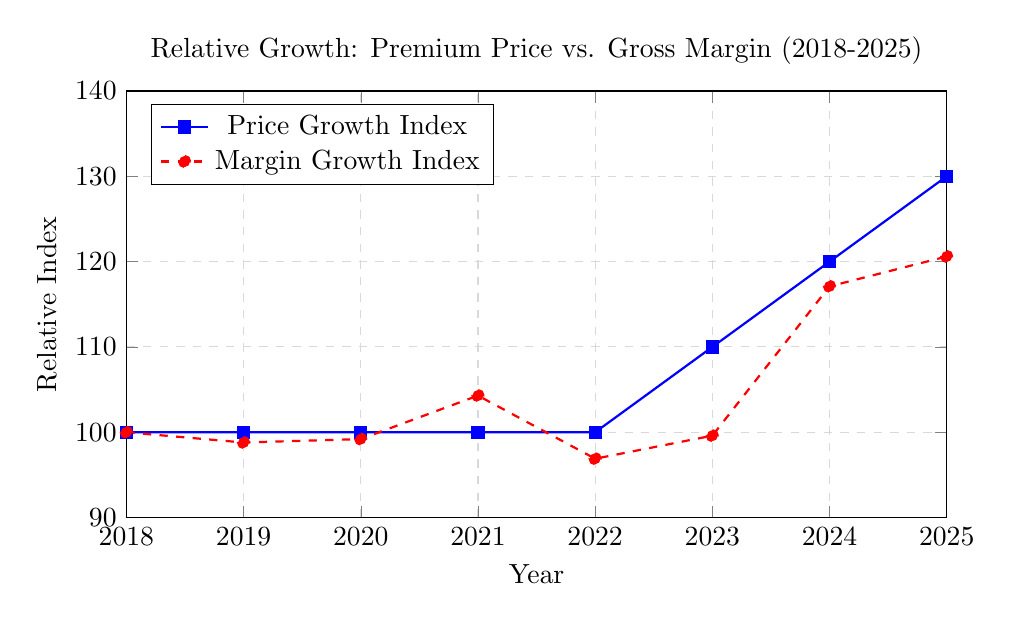
\begin{tikzpicture}
        \begin{axis}[
            width=12cm, height=7cm,
            xmin=2018, xmax=2025,
            ymin=90, ymax=140,
            xtick={2018, 2019, 2020, 2021, 2022, 2023, 2024, 2025},
            x tick label style={/pgf/number format/1000 sep=},
            ytick={90, 100, 110, 120, 130, 140},
            ylabel={Relative Index},
            xlabel={Year},
            title={Relative Growth: Premium Price vs. Gross Margin (2018-2025)},
            legend pos=north west,
            grid=both,
            grid style={dashed, gray!30}
        ]

        % Price Indexed: (Current Price / 9.99) * 100
        \addplot[
            color=blue,
            mark=square*,
            thick
        ] coordinates {
            (2018, 100.0)
            (2019, 100.0)
            (2020, 100.0)
            (2021, 100.0)
            (2022, 100.0)
            (2023, 110.0) % 10.99 / 9.99
            (2024, 120.0) % 11.99 / 9.99
            (2025, 130.0) % 12.99 / 9.99
        };
        \addlegendentry{Price Growth Index}

        % Margin Indexed: (Current Margin / 25.7) * 100
        \addplot[
            color=red,
            mark=*,
            thick,
            dashed
        ] coordinates {
            (2018, 100.0)
            (2019, 98.8)  % 25.4 / 25.7
            (2020, 99.2)  % 25.5 / 25.7
            (2021, 104.3) % 26.8 / 25.7
            (2022, 96.9)  % 24.9 / 25.7
            (2023, 99.6)  % 25.6 / 25.7
            (2024, 117.1) % 30.1 / 25.7
            (2025, 120.6) % 31.0 / 25.7
        };
        \addlegendentry{Margin Growth Index}

        \end{axis}
    \end{tikzpicture}
    \caption{Relative growth index of Spotify's Premium Price \cite{spotify_prices} and Gross Profit Margin \cite{spotify_gross_margin}, normalised to a base value of 100 in the year 2018.}
    \label{fig:spotify_economics_indexed}
\end{figure}

\par In an effort to ease the load on cloud infrastructure, the academic community has explored decoupled network models, including hybrid CDN-P2P systems and peer-assisted CDNs \cite{hybrid_cdn_p2p,pa_cdn_survey}. Translating these architectures into a working system, however, means meeting the same recurring design problems. The system has to hide latency so playback starts when the listener presses play, even though peers still have to be found and connected. It has to establish direct peer-to-peer links across NATs, firewalls and the browser security sandbox, on native and web platforms alike. It has to decide what the client stores and for how long, balancing network offload against device storage and battery. It has to segment and verify audio so that bytes from an untrusted peer are as safe as bytes from the server. Finally, it has to react to fluctuating peer performance without stalling playback or fragmenting the shared data across the swarm.

\par Each of the following sections takes one of these domains in turn and weighs the leading candidate solutions against each other. The order roughly follows the path of a single chunk through the system, from the moment playback is requested to the moment the bytes are verified and played. None of the domains is treated in isolation, because a decision taken in one of them quietly constrains the choices left in the others. A final section then steps back to look at how complete systems have combined these choices in practice.

\section{Achieving Near-Instant Playback}
\indent \par The first requirement of a modern streaming service is simple to state and hard to satisfy: playback has to start quickly. A listener who presses play does not think about peer discovery, buffer maps or NAT traversal. They expect sound, and they expect it now. A system that is correct in every other respect but slow to start will still feel broken, so this requirement has to be satisfied before any of the others can matter.

\par A download-first approach is therefore a bad fit for streaming. If a listener has to wait for the whole file, even a technically correct system feels broken. Research on Quality of Experience (QoE) supports the same intuition: in the large-scale study by Krishnan and Sitaraman, users begin abandoning streaming content rapidly when startup delays exceed only a few seconds, with the penalty becoming visible around the two-second mark \cite{quality_impact}. The lesson is that startup latency is not a secondary metric to be tuned later, but a hard constraint that shapes the delivery architecture from the outset.

\begin{figure}[htbp]
    \centering
    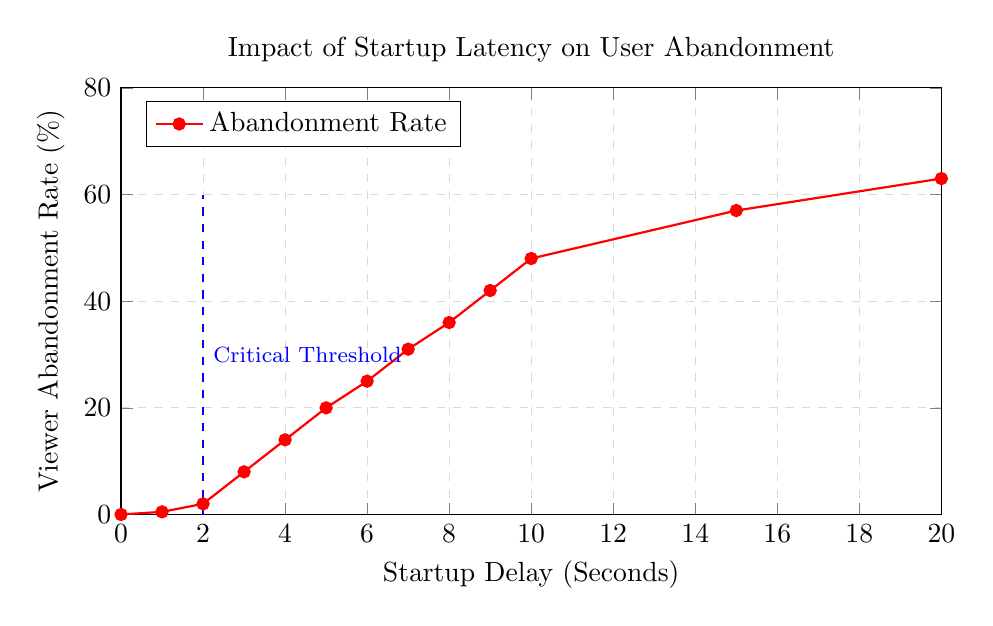
\begin{tikzpicture}
        \begin{axis}[
            width=12cm, height=7cm,
            xlabel={Startup Delay (Seconds)},
            ylabel={Viewer Abandonment Rate (\%)},
            xmin=0, xmax=20,
            ymin=0, ymax=80,
            grid=both,
            grid style={dashed, gray!30},
            title={Impact of Startup Latency on User Abandonment},
            legend pos=north west
        ]

        \addplot[
            color=red,
            mark=*,
            thick
        ] coordinates {
            (0, 0)
            (1, 0.5)
            (2, 2)
            (3, 8)
            (4, 14)
            (5, 20)
            (6, 25)
            (7, 31)
            (8, 36)
            (9, 42)
            (10, 48)
            (15, 57)
            (20, 63)
        };
        \addlegendentry{Abandonment Rate}

        \draw[dashed, thick, blue] (axis cs:2,0) -- (axis cs:2,60) node[midway, right, font=\footnotesize] {Critical Threshold};

        \end{axis}
    \end{tikzpicture}
    \caption{Viewer abandonment rate as a function of startup delay\cite{quality_impact}.}
    \label{fig:latency_abandonment}
\end{figure}

\par The architecture therefore has to use progressive delivery. The listener should perceive near-instant playback, while the system quietly prepares the slower parts of the delivery path in the background. Both of the techniques below try to remove the wait the listener would otherwise see, but they place that preparatory work at different points in time and pay for it in different ways. The two main strategies considered here are prefix caching and predictive pre-fetching.

\subsection{Prefix Caching}
\indent \par Prefix caching means that the server immediately sends the first part of the content while the P2P connection is established in the background for the rest. The idea is well known in multimedia proxy work: by storing the first seconds of a clip, the proxy can hide the delay and throughput variation of the slower path \cite{prefix_caching}. The first part of the file is the only segment whose timing the listener perceives directly, so guaranteeing it from a fast, reliable source is enough to make playback feel instant. Everything after it can be assembled more slowly, as long as it arrives before the prefix runs out.

\par This method gives the user a reliable start from the server and masks the P2P connection setup time. It also absorbs the initial demand burst and acts as a fail-safe, because the server can continue streaming the whole track if peers are unavailable. The downside is that prefix caching adds server storage and byte-range complexity, and it creates one sensitive boundary: the transition from the server prefix to the peer-supplied chunks. If that transition is not synchronised, the listener may hear clicks, silence or other artefacts.

\subsection{Predictive Pre-Fetching}
\indent \par Predictive pre-fetching is, at least on paper, a good alternative to prefix caching. It uses a prediction model to guess the user's next choice, then downloads that content in the background before the user reaches it. The wait disappears entirely when the guess is correct, because the content is already on the device by the time it is requested. The whole approach therefore rises or falls on the quality of the prediction, which is where its weaknesses appear.

\par This method can remove the buffering issue, keep startup delay close to zero, and even allow offline playback if the connection drops after the content was fetched. It also brings obvious waste. The client may fill storage with media the user never plays, the system may consume bandwidth for wrong predictions, and the cloud may still pay for bytes that helped nobody. As evaluated by Krishnamoorthi et al., pre-fetching can reduce startup time for likely next videos, but only when the client carefully balances aggressiveness against bandwidth use and the quality of the video that is already playing \cite{bandwidth_aware_prefetching}.


\begin{figure}[htbp]
    \centering
    \begin{tikzpicture}[
        node distance=2cm,
        box/.style={draw, rectangle, minimum width=3cm, minimum height=1.2cm, align=center, fill=gray!10, rounded corners},
        arrow/.style={->, >=Stealth, thick},
        label_text/.style={font=\footnotesize\itshape}
    ]
        \node[font=\bfseries] (title_prefix) at (0, 3.5) {Prefix Caching Model};
        \node[box] (server_prefix) at (-2, 2) {Master Server\\(5\% Prefix)};
        \node[box] (peer_prefix) at (2, 2) {P2P System\\(95\% Suffix)};
        \node[box, fill=blue!10] (buffer_prefix) at (0, 0) {Client Audio Buffer\\(Instant Playback)};

        \draw[arrow] (server_prefix) -- node[left, label_text] {Immediate TCP} (buffer_prefix);
        \draw[arrow] (peer_prefix) -- node[right, label_text] {Background UDP} (buffer_prefix);

        \node[font=\bfseries] (title_predict) at (8, 3.5) {Predictive Pre-Fetching Model};
        \node[box] (network_predict) at (8, 2) {Network Sources\\(Server or Peers)};
        \node[box, fill=red!10] (storage_predict) at (8, 0) {Client Persistent Storage\\(Full 100\% File Cache)};
        \node[box, fill=blue!10] (buffer_predict) at (8, -2.5) {Client Audio Buffer\\(Eventual Playback)};

        \draw[arrow] (network_predict) -- node[right, label_text] {Background Download} (storage_predict);
        \draw[arrow] (storage_predict) -- node[right, label_text] {Local Disk Read} (buffer_predict);
        \draw[thick, dotted, gray] (4, -3.5) -- (4, 4);

    \end{tikzpicture}
    \caption{Data-flow comparison of Prefix Caching vs Predictive Pre-Fetching.}
    \label{fig:caching_comparison}
\end{figure}

\section{Bridging Native And Browser Environments}
\indent \par Peer-assisted streaming only works if peers can actually reach each other. That sounds obvious, but it becomes difficult when the same application has to run both as a native program and inside a web browser. Native operating systems expose socket APIs that allow direct access to TCP and UDP \cite{top_down_cn}. Browsers, for good security reasons, do not.

\par A system that uses one networking protocol on native clients and another in the browser is fragile from the start. The browser sandbox forbids arbitrary sockets to untrusted peers, because otherwise a web page would become a very convenient attack tool \cite{webrtc_security}. Rescorla's WebRTC security architecture makes the same point plainly: without protocol-level cryptographic safeguards, unauthenticated peers cannot be trusted \cite{webrtc_security}. In this context, an architecture that cannot merge native and browser clients cannot deliver cross-platform P2P streaming at all.

\par The transport therefore has to navigate complex network topologies without violating the security model of any platform. The system needs one peer swarm, not a desktop swarm, a mobile swarm and a browser island. A fragmented swarm would split the pool of peers holding any given chunk, which directly weakens the offload the whole design depends on. The main candidate for this role is Web Real-Time Communication (WebRTC), with relay-only delivery through TURN or proxy servers kept as the contrasting option.

\subsection{Web Real-Time Communication (WebRTC)}
\indent \par WebRTC offers mandatory security through Datagram Transport Layer Security (DTLS) and includes built-in Network Address Translation (NAT) traversal mechanisms such as Interactive Connectivity Establishment (ICE, not to be confused with whatever the USA is doing nowadays) and Session Traversal Utilities for NAT (STUN). The W3C WebRTC Recommendation standardises the browser API for exchanging media and generic application data between browsers or compatible devices, while ICE itself is defined as the NAT traversal procedure that searches for a usable path between peers \cite{webrtc_w3c,ice_rfc8445}. The decisive property for this thesis is that the same standard is implemented by every major browser and by the native libraries the client uses, so a single connection model works across all the target platforms. Connectivity and security therefore come from the protocol itself rather than from anything the application has to build by hand.

\par This lets devices on private networks communicate over the public internet without browser plugins. For this thesis, the important part is the DataChannel: the IETF specification places generic peer data on SCTP over DTLS, which is exactly the reliable ordered transport needed for chunk requests and responses \cite{webrtc_data_channels}. WebRTC is not perfect, though. It adds connection setup overhead, consumes CPU on the client, and requires a signaling server to coordinate the offer, answer and ICE candidate exchange (see Figure \ref{fig:webrtc_architecture}). Researchers at Universidad Rey Juan Carlos measured mean latencies of around 200 ms without packet loss and around 400 ms in a second experiment, while also noting that the UDP-based approach loses scalability when many clients are introduced \cite{webrtc_testing}.

\begin{figure}[htbp]
    \centering
    \begin{tikzpicture}[
        node distance=2.5cm,
        client/.style={draw, rectangle, minimum width=2.5cm, minimum height=1.5cm, align=center, fill=blue!10, rounded corners},
        server/.style={draw, rectangle, minimum width=2.5cm, minimum height=1.5cm, align=center, fill=gray!20, rounded corners},
        arrow/.style={->, >=Stealth, thick},
        biarrow/.style={<->, >=Stealth, thick},
        label_text/.style={font=\footnotesize\itshape}
    ]

        \node[client] (peerA) at (0, 0) {Peer A\\(NAT A)};
        \node[client] (peerB) at (8, 0) {Peer B\\(NAT B)};

        \node[server] (signaling) at (4, 3) {Signaling Server\\(SDP Exchange)};
        \node[server] (stun) at (4, -3) {STUN Server\\(IP Discovery)};

        \draw[biarrow, dashed] (peerA) -- node[above left, label_text] {WebSocket} (signaling);
        \draw[biarrow, dashed] (peerB) -- node[above right, label_text] {WebSocket} (signaling);

        \draw[biarrow, dotted] (peerA) -- node[below left, label_text] {UDP Binding} (stun);
        \draw[biarrow, dotted] (peerB) -- node[below right, label_text] {UDP Binding} (stun);

        \draw[biarrow, draw=green!60!black, line width=1.5pt] (peerA) -- node[above, font=\bfseries\footnotesize] {Direct WebRTC Media} (peerB);

    \end{tikzpicture}
    \caption{WebRTC architecture.}
    \label{fig:webrtc_architecture}
\end{figure}

\subsection{'Relay-Only' (TURN/Proxy Servers)}
\indent \par Relay-only delivery takes the opposite route. It guarantees connectivity by routing all P2P traffic through Traversal Using Relays around NAT (TURN) or proxy servers (see Figure \ref{fig:turn_architecture}). TURN provides a reliable relay for peers behind restrictive symmetric NATs or enterprise firewalls that block direct UDP communication \cite{relays_turn}. Because the relay sits in the data path for every transfer, connectivity stops being a question the application has to solve case by case, which is the entire appeal of the approach.

\par This simplifies the client and makes connection monitoring easier, but it also moves the bandwidth bill back to infrastructure controlled by the provider. Every relayed byte is paid for like a server byte, which weakens the main reason for using P2P in the first place. It also adds a central point of failure to the P2P component, which is especially undesirable for content streaming. For a system whose whole purpose is to push bytes off the provider's infrastructure, a transport that routes those same bytes back through it is self-defeating, which is why this thesis keeps TURN only as a conceptual contrast and never relies on it.

\begin{figure}[htbp]
    \centering
    \begin{tikzpicture}[
        node distance=3cm,
        client/.style={draw, rectangle, minimum width=3cm, minimum height=1.5cm, align=center, fill=blue!10, rounded corners, font=\bfseries},
        server/.style={draw, rectangle, minimum width=3.5cm, minimum height=2cm, align=center, fill=red!10, rounded corners, font=\bfseries},
        arrow/.style={->, >=Stealth, thick, draw=red!60!black, line width=1.5pt},
        label_text/.style={font=\small\itshape, align=center, fill=white, inner sep=2pt}
    ]
        \node[client] (peerA) at (0, 0) {Peer A\\(Symmetric NAT)};
        \node[client] (peerB) at (10, 0) {Peer B\\(Symmetric NAT)};
        \node[server] (turn) at (5, 2) {TURN Server\\(Centralized Bandwidth Proxy)};

        \draw[arrow] (peerA) to[bend left=25] node[above, label_text, pos=0.0] {1. Upload Media} (turn);
        \draw[arrow] (turn) to[bend left=20] node[above, label_text, pos=0.0] {2. Relay to B} (peerB);
        \draw[arrow] (peerB) to[bend left=20] node[below, label_text, pos=0.5] {3. Upload Media} (turn);
        \draw[arrow] (turn) to[bend left=20] node[below, label_text, pos=0.5] {4. Relay to A} (peerA);

    \end{tikzpicture}
    \caption{Relay-Only (TURN) architecture.}
    \label{fig:turn_architecture}
\end{figure}

\section{Balancing Efficiency and Device Constraints}
\indent \par A distributed streaming system also has to decide if, how and when data is kept on the consumer device. This choice balances network efficiency for the provider and the listener against the storage and battery limits of the device. It also determines whether a listener can act as a source for others later, since a device can only serve a chunk it still holds. The two client-side retention strategies considered here are mobile edge caching and ephemeral RAM caching.

\subsection{Mobile Edge Caching}
\indent \par Mobile edge caching stores data semi-permanently on the persistent storage of the client. By keeping content locally, the device becomes a potential edge peer, capable of both consuming data and serving cached data to other devices. The cached copy outlives the playback session that produced it, so it remains available for a later listen or a later peer request. This persistence is what turns an ordinary client into a durable node in the delivery network.

\par The main advantage is the reduction of redundant network traffic and centralised infrastructure cost. If a media file is kept on the client's disk, a later playback by the same user can be served locally, bypassing the network completely. The same cached file can also be served to other peers, turning the listener into a node in the P2P network and offloading expensive egress bandwidth for the provider. The benefit grows with the popularity of a track, because each additional listener that retains it adds another potential source for the next one.

\par These networking benefits have costs. Downloading may conserve energy compared with repeated network fetches, but uploading to other devices can drain the client's battery. Asadi et al. highlight this duality in their survey of Device-to-Device communication, noting that D2D offloading reduces congestion and traffic but shifts part of the energy burden to the cooperating user equipment \cite{d2d_survey}. Peers are also human-owned devices: they lose network connectivity, enter sleep mode, or have the application terminated by the operating system, creating a risk of mid-stream interruption for the downloader. Finally, to prevent local storage exhaustion, this approach needs a cache eviction policy, such as deleting older media based on age, size or play frequency.

\subsection{Ephemeral RAM Caching}
\indent \par Ephemeral RAM caching keeps the chunks of the currently playing media only in the client's Random Access Memory (RAM). The data is evicted as soon as the track finishes or is skipped by the user. Nothing is ever written to persistent storage, so the cache lives and dies with the playback session that created it. The device holds only what it is actively listening to, and forgets it the moment that listening stops.

\par The main advantage is that no data is saved in persistent storage. Storage exhaustion stops being a concern, and the implementation becomes simpler because it no longer needs storage management, eviction heuristics or storage permission requests. There is also nothing to clean up when the application closes, since the operating system reclaims the memory automatically. This makes the approach attractive on platforms where persistent storage is restricted or unavailable, such as the browser.

\par The simplification comes at the expense of the P2P network. Downloading the same bytes again and again wastes bandwidth, and keeping more in RAM quickly runs into device limits or operating-system pressure. Liang et al. describe how mobile systems use mechanisms such as the Low Memory Killer (LMK) and background reclaim daemons (kswapd) to terminate background applications when memory pressure rises \cite{apps_performance_diffs}. Most importantly, because the data is transient, the device can rarely be used as a reliable node for other peers, which removes much of the value of the P2P layer.

\begin{figure}[htbp]
    \centering
    \begin{tikzpicture}[
        node distance=2cm,
        client/.style={draw, rectangle, minimum width=2.8cm, minimum height=1.2cm, align=center, fill=gray!10, rounded corners},
        storage/.style={draw, cylinder, aspect=0.3, minimum width=2.5cm, minimum height=1.5cm, align=center, fill=blue!10, shape border rotate=90},
        ram/.style={draw, rectangle, minimum width=2.5cm, minimum height=1.5cm, align=center, fill=red!10, dashed},
        arrow/.style={->, >=Stealth, thick}
    ]
        \node[font=\bfseries] (title_edge) at (0, 4.5) {Mobile Edge Caching};

        \node[client] (net_edge) at (0, 3) {Network Download};
        \node[storage] (disk) at (0, 0.5) {Persistent\\Disk Storage};

        \node[client] (play_edge) at (-2, -2) {Audio Player};
        \node[client, fill=green!10] (peer_edge) at (2, -2) {Other P2P Peers};

        \draw[arrow] (net_edge) -- (disk);

        \draw[arrow] (disk.south) -- (0, -0.5) -- (-2, -0.5) -- (play_edge.north);
        \draw[arrow] (disk.south) -- (0, -0.5) -- (2, -0.5) -- node[right, font=\footnotesize\itshape, align=left] {Served as\\Edge Node} (peer_edge.north);

        \node[font=\bfseries] (title_ram) at (8.5, 4.5) {Ephemeral RAM Caching};

        \node[client] (net_ram) at (8.5, 3) {Network Download};
        \node[ram] (ram_node) at (8.5, 0.5) {Volatile\\RAM Buffer};

        \node[client] (play_ram) at (6.5, -2) {Audio Player};
        \node[client, fill=gray!30, text=gray] (peer_ram) at (10.5, -2) {Other P2P Peers};

        \draw[arrow] (net_ram) -- (ram_node);

        \draw[arrow] (ram_node.south) -- (8.5, -0.5) -- (6.5, -0.5) -- (play_ram.north);
        \draw[arrow, dashed, draw=red!70] (ram_node.south) -- (8.5, -0.5) -- (10.5, -0.5) -- node[midway, text=red, font=\Huge\bfseries] {$\times$} (peer_ram.north);

        \node[font=\footnotesize\itshape, text=red, align=center] at (11, 0) {Data evicted;\\Cannot serve};

        \draw[thick, dotted, gray] (4.5, -3.5) -- (4.5, 5);

    \end{tikzpicture}
    \caption{Data flow comparison of Mobile Edge Caching vs Ephemeral RAM Caching.}
    \label{fig:storage_comparison}
\end{figure}

\section{Syncing and Integrity}
\indent \par The next decision is how the media file is structured during transfer. This choice determines how the file is segmented, exchanged, verified and recovered after failure. It also decides whether parallel downloading is possible at all. The two options considered here are chunk-based synchronization and continuous byte-stream transmission.


\subsection{Chunk-Based Synchronization}
\indent \par Under the chunk-based synchronization model, the complete file is deterministically split into small, fixed-size pieces. Data transfer and P2P exchange then happen at the granularity of these chunks. This approach provides strong data verification and fault tolerance, because each chunk has its own cryptographic checksum and only a corrupted chunk has to be downloaded again (see Figure \ref{fig:chunk_based_sync}). A good checksum for this verification is SHA-256, part of the NIST Secure Hash Standard, which makes the integrity rule independent of the peer that supplied the bytes \cite{secure_hash_standard}. The same structure enables parallel downloading: the client can request different chunks from multiple peers and increase total throughput. As established by Cohen's foundational BitTorrent architecture, distributing data in cryptographically verified pieces not only protects file integrity against malicious or faulty nodes, but also enables swarming, where a client downloads disjoint chunks from many independent sources \cite{bittorent}. This approach also facilitates deduplication, because the network can identify and share identical chunks across peers.

\begin{figure}[htbp]
    \centering
    \begin{tikzpicture}[
        node distance=1.5cm,
        peer/.style={draw, circle, minimum size=1.2cm, align=center, fill=green!10, font=\footnotesize\bfseries},
        client/.style={draw, rectangle, minimum width=3cm, minimum height=1.5cm, align=center, fill=blue!10, rounded corners, font=\bfseries},
        arrow/.style={->, >=Stealth, thick},
        error_arrow/.style={->, >=Stealth, thick, dashed, draw=red},
        label_text/.style={font=\scriptsize\itshape, align=center, text=red}
    ]

        \node[peer] (peer1) at (0, 3) {Peer 1};
        \node[peer] (peer2) at (3, 3) {Peer 2};
        \node[peer] (peer3) at (6, 3) {Peer 3};
                \node[client] (client_chunk) at (3, 0) {Client Buffer\\(Reassembly \& Verification)};

        \draw[arrow] (peer1.south) -- node[left, font=\scriptsize] {Chunk 1 (OK)} (client_chunk.north west);
        \draw[error_arrow] (peer2.south) -- node[right, font=\scriptsize, align=left, text=red] {Chunk 2 (Corrupted)} (client_chunk.north);
        \draw[arrow] (peer3.south) -- node[right, font=\scriptsize] {Chunk 3 (OK)} (client_chunk.north east);

        \node[label_text] at (3, -1.5) {Fault Isolated: Only Chunk 2 is discarded\\and re-requested from another peer.};

    \end{tikzpicture}
    \caption{Chunk-Based Synchronization, corruption is isolated to individual segments.}
    \label{fig:chunk_based_sync}
\end{figure}

\par The cost is protocol overhead. Every chunk needs its own request and response, with transport headers and request identifiers. The client also has to maintain a real-time state map that tracks which chunks are downloaded, in transit or missing. Finally, the chunks must be reassembled in the correct order for gapless playback, which introduces strict buffer-management requirements at the application layer. As demonstrated by Zhang et al. in their data-driven P2P streaming network, this approach requires the active exchange of local 'Buffer Maps' between nodes and aggressive chunk scheduling so pieces arrive before their playback deadlines \cite{coolstreaming}.

\subsection{Continuous Byte-Stream}
\indent \par As an alternative, the continuous byte-stream approach treats the entire file as a single, contiguous pipe of data, mirroring traditional HTTP progressive streaming. The main advantage is low protocol overhead. Because the data is transmitted as a single continuous stream, the system avoids repetitive headers, request IDs and per-chunk checksums. The playback logic also becomes simpler, because the media player pulls data sequentially from a linear stream buffer without complex reordering.

\begin{figure}[htbp]
    \centering
    \begin{tikzpicture}[
        node distance=2cm,
        peer/.style={draw, circle, minimum size=1.5cm, align=center, fill=purple!10, font=\footnotesize\bfseries},
        client/.style={draw, rectangle, minimum width=3cm, minimum height=1.5cm, align=center, fill=purple!10, rounded corners, font=\bfseries},
        arrow/.style={->, >=Stealth, ultra thick},
        label_text/.style={font=\scriptsize\itshape, align=center, text=red}
    ]

        \node[peer] (peer_source) at (0, 4.5) {Single Source\\Peer};

        \node[client] (client_stream) at (0, 0) {Client Buffer\\(Linear Read)};

        \draw[arrow] (peer_source.south) -- node[pos=0.5, left, font=\scriptsize, align=right, text=black] {Monolithic Byte-Stream\\(No parallelism)} (0, 2.05);

        \draw[ultra thick, red] (-0.15, 2.05) -- (0.15, 1.75);
        \draw[ultra thick, red] (-0.15, 1.75) -- (0.15, 2.05);
        \node[font=\bfseries, text=red, right] at (0.5, 1.9) {Data Corruption};

        \draw[ultra thick, red, dashed, ->, >=Stealth] (0, 1.75) -- (client_stream.north);

        \node[label_text] at (0, -1.5) {Fragile Integrity: A single error invalidates\\the entire stream from that point onward.};

    \end{tikzpicture}
    \caption{Continuous Byte-Stream fragile single point of failure}
    \label{fig:continuous_stream_failure}
\end{figure}

\par Despite the simplicity, this method is incompatible with the core mechanics of a robust peer-assisted network. The monolithic structure prevents parallel downloading, because the client is effectively tied to one source at a time. More importantly, integrity becomes fragile (see Figure \ref{fig:continuous_stream_failure}). If one byte in the stream is corrupted or lost, the integrity of the file from that point onward is compromised. This is a realistic concern in a P2P system, where peer sessions can be short and unstable \cite{measurement_p2p}. Without granular checksums to isolate the error, the client may have to discard the received buffer and restart from a safe point, which is unacceptable for interactive playback.


\section{Managing Quality and Source Selection}
\indent \par Network conditions fluctuate constantly during streaming, so the distributed system needs a flow-control strategy. That strategy has to watch the current network conditions and decide how to avoid playback stalls. The two candidates differ in what they sacrifice when bandwidth drops: one lowers the quality of the audio, the other changes where the audio comes from. The two main options are adaptive bitrate and adaptive routing.

\subsection{Adaptive Bitrate}
\indent \par Adaptive Bitrate (ABR) dynamically changes the quality, and therefore the bitrate, of the content being streamed, based on the client's connection speed and buffer health. This approach is the established industry standard for centralised video streaming services such as YouTube and Netflix. As detailed by Stockhammer in the foundational specification of DASH (Dynamic Adaptive Streaming over HTTP), ABR breaks media into segments encoded at several bitrates, allowing the client to request the best representation for the current bandwidth \cite{standards_streaming_http}. HTTP Live Streaming follows the same family of ideas through variant streams that clients switch between based on network conditions \cite{hls_rfc8216}.


\par Its main advantage is playback continuity. By reducing the bitrate when bandwidth drops, the system lowers the chance of re-buffering and keeps the data rate close to the available network capacity. The stream therefore keeps flowing even on a degraded connection, where a fixed-quality stream would stall and re-buffer. The listener trades fidelity for the absence of interruptions, which is usually the right trade for video.

\par The drawback is that quality changes can be noticeable, especially in music if the representation switch affects perceived fidelity. From a provider perspective, ABR also complicates P2P sharing. The client has to manage a multidimensional chunk map that tracks both the chunk and its quality level, which makes peer discovery and deduplication much harder. The master server also has to compute and store multiple representations of every media file, increasing centralised storage cost. Figure \ref{fig:abr_fragmentation} illustrates the problem.

\begin{figure}[htbp]
    \centering
    \begin{tikzpicture}[
        node distance=1.5cm,
        peer/.style={draw, circle, minimum size=1.5cm, align=center, fill=gray!10, font=\footnotesize\bfseries},
        chunk/.style={draw, rectangle, minimum width=2.5cm, minimum height=0.6cm, align=center, font=\scriptsize\bfseries},
        arrow/.style={->, >=Stealth, thick},
        label_text/.style={font=\scriptsize\itshape, align=center, text=red}
    ]

        \node[draw, rectangle, fill=blue!10, minimum width=4.5cm, minimum height=4cm, rounded corners] (server_box) at (0, 3.2) {};

        \node[align=center, font=\bfseries] (server_text) at (0, 4.6) {Master Server};

        \node[chunk, fill=green!20] (high) at (0, 3.7) {Chunk 1 (1080p)};
        \node[chunk, fill=yellow!20] (med) at (0, 2.9) {Chunk 1 (720p)};
        \node[chunk, fill=red!20] (low) at (0, 2.1) {Chunk 1 (360p)};

        \node[peer] (peer1) at (-3.5, -1) {Peer A};
        \node[peer] (peer2) at (3.5, -1) {Peer B};

        \node[chunk, fill=red!20] (peer1_chunk) at (-3.5, -2.5) {Chunk 1 (360p)};
        \node[chunk, fill=green!20] (peer2_chunk) at (3.5, -2.5) {Chunk 1 (1080p)};

        \draw[arrow, dashed, draw=red] (low.west) to[bend right=20] node[left, font=\scriptsize, align=center, xshift=-0.1cm] {Slow\\Network} (peer1.north);
        \draw[arrow, dashed, draw=green!60!black] (high.east) to[bend left=20] node[right, font=\scriptsize, align=center, xshift=0.1cm] {Fast\\Network} (peer2.north);

        \draw[<->, >=Stealth, ultra thick, draw=red] (peer1_chunk.east) -- node[above, font=\bfseries] {Hash Mismatch} node[below, font=\scriptsize\itshape] {Cannot Share} (peer2_chunk.west);

    \end{tikzpicture}
    \caption{Adaptive Bitrate example of failing peer-to-peer de-duplication.}
    \label{fig:abr_fragmentation}
\end{figure}

\subsection{Adaptive Routing}
\indent \par Alternatively, Adaptive Routing requires that the chosen quality remains strictly constant for the entire duration of the playback. If the current peer cannot sustain the required data flow, the system does not drop the quality, it immediately switches the download source. The client dynamically reroutes its chunk requests to a faster peer or, as an absolute last resort, falls back to the central Master Server to maintain the established bitrate (see Figure \ref{fig:adaptive_routing_switch}). The variable that absorbs network fluctuation is therefore the source of the bytes rather than their quality, which keeps the listening experience constant regardless of which peer happens to be supplying the audio at any given moment.

\par The most significant benefit of this approach is consistent quality. The user's experience is defined strictly by the fidelity they initially selected, maintaining client control regardless of network fluctuations. Architecturally, fixed-bitrate routing simplifies de-duplication and checksum verification. Because the quality is immutable, a specific chunk is mathematically identical across the entire P2P network, ensuring that cryptographic checksums always match and facilitating peer discovery logic.

\begin{figure}[htbp]
    \centering
    \begin{tikzpicture}[
        node distance=2cm,
        peer_red/.style={draw, circle, minimum size=1.5cm, align=center, fill=red!10, font=\footnotesize\bfseries},
        peer_green/.style={draw, circle, minimum size=1.5cm, align=center, fill=green!10, font=\footnotesize\bfseries},
        client/.style={draw, rectangle, minimum width=3cm, minimum height=1.5cm, align=center, fill=blue!10, rounded corners, font=\bfseries},
        arrow/.style={->, >=Stealth, thick},
        fail_arrow/.style={->, >=Stealth, thick, dashed, draw=red},
        label_text/.style={font=\scriptsize\itshape, align=left}
    ]
        \node[peer_red] (peer1) at (-2.5, 3) {Peer 1\\(Failing)};
        \node[peer_green] (peer2) at (2.5, 3) {Peer 2\\(Healthy)};
        \node[draw, rectangle, fill=gray!20, minimum width=2cm, minimum height=1cm, align=center, rounded corners, font=\scriptsize\bfseries] (server) at (6, 3) {Master Server};

        \node[client] (client_routing) at (0, 0) {Client Buffer};

        \draw[fail_arrow] (peer1.south) -- node[left, label_text, text=red] {Throughput Drop\\Detected} (client_routing.north west);
        \draw[arrow, draw=green!60!black] (peer2.south) -- node[right, label_text, text=green!40!black] {Preemptive\\Source Switch} (client_routing.north east);
        \draw[arrow, dotted, draw=gray] (server.south) |- node[above right, font=\scriptsize, pos=0.8] {Standby HTTP Fallback} (client_routing.east);

    \end{tikzpicture}
    \caption{Adaptive Routing data source switching.}
    \label{fig:adaptive_routing_switch}
\end{figure}

\par The cost of this strict quality rule is a higher risk of interruption. When a peer fails, the system has to switch sources quickly. If the routing switch takes too long, or if the replacement source also has insufficient bandwidth, playback stalls and the client has to re-buffer. As Magharei et al. demonstrated in their comparative study of P2P streaming architectures, maintaining continuous playback under these constraints requires a mesh-pull mechanism: the client must maintain a dynamic pool of standby neighbours and use aggressive chunk scheduling to request missing segments before the active playback buffer drains \cite{live_p2p_approaches}. The client therefore needs stricter buffer management and peer-performance prediction, and the central server still has to act as the final fail-safe when several peers fail at once.


\section{Lessons from Prior Peer-Assisted Systems}
\indent \par The five domains dissected above are not a checklist invented for this thesis. Every one of them was confronted, in some form, by the peer-assisted systems that came before it. Stepping back from the individual trade-offs to look at how complete systems combined them is instructive in two ways. It confirms that peer assistance is a proven technique rather than a speculative one, and it exposes precisely which of the older assumptions no longer hold under the browser, mobile and cloud constraints that this work targets.

\subsection{BitTorrent}
\indent \par The foundational reference point is BitTorrent, whose architecture Cohen described as a swarm of peers exchanging fixed-size, cryptographically identified pieces \cite{bittorent}. BitTorrent established the result that a population of downloaders can collectively serve a file with the origin contributing little more than the first complete copy, and that content-addressed pieces let a client assemble that file from many untrusted sources without sacrificing integrity. What it deliberately does not provide is any notion of a playback deadline: a torrent is finished when every piece has arrived, in whatever order, which is acceptable for a bulk download but not for a listener who expects sound the instant a track is clicked.

\subsection{CoolStreaming}
\indent \par CoolStreaming narrowed that gap for live media. Zhang et al. built a data-driven mesh in which peers periodically exchange 'buffer maps' advertising the segments they hold and pull missing segments from whichever partner can meet the playback deadline \cite{coolstreaming}. This demonstrated that a mesh-pull design can sustain media under real-time constraints, and it is the direct ancestor of the buffer-map peer discovery and deadline-aware chunk scheduling that reappear later in this thesis. Its assumptions, however, are those of live broadcast: a single shared timeline across all viewers, desktop clients on relatively stable connections, and a tolerance for several seconds of startup buffering that an on-demand music player cannot afford.

\subsection{Old Spotify}
\indent \par The closest precedent of all is Spotify's old production system. Kreitz and Niemel\"a measured a low-latency, peer-assisted music-on-demand architecture serving a large user base, in which the server delivered the beginning of each track and stood by as a fallback while peers supplied the remainder \cite{spotify_p2p}. The shape of that design, a server-seeded prefix, a peer swarm for the bulk of the bytes, and an origin fallback, is almost the same shape that the preceding sections kept arguing toward, which is reassuring: the architecture is known to work at scale. The follow-up work on integrating smartphones into the same model is equally instructive in the opposite direction, showing that mobile devices cannot be treated as desktop peers because battery state, radio access and aggressive background termination change what a peer can promise \cite{spotify_mobile_p2p}. Spotify ultimately retired its peer-assisted layer in favour of a pure cloud and CDN path, a decision driven less by any flaw in the model than by the operational simplicity of centralisation and the rise of the web client, which at the time had no way to open peer connections at all. The lesson this thesis takes from that history is that the model was never the problem, the platforms were, and the platform that made peer assistance impossible in the browser is precisely the one that WebRTC has since reopened.

\subsection{Hybrid CDN-P2P and Peer-Assisted CDNs}
\indent \par This reading is consistent with the broader academic treatment of the subject. Surveys of hybrid CDN-P2P and peer-assisted CDN architectures converge on the same division of labour, with the centralised infrastructure shrinking to a seeder and a guarantor of availability rather than the source of every byte \cite{hybrid_cdn_p2p,pa_cdn_survey}. On the cellular side, the device-to-device offloading literature frames the same exchange in terms of relieving network congestion at the cost of energy on the cooperating handset \cite{d2d_survey}, while long-running measurement studies of deployed peer populations supply the churn figures that any realistic cost estimate has to respect \cite{measurement_p2p}.


\indent \par Taken together, these systems establish two things that the rest of the thesis builds on. The origin is not eliminated but demoted, and the engineering problem is to make its role as small as the constraints allow. The five design choices are not independent knobs but a coupled system, in which a commitment in one domain closes options in the others. What the prior work does not supply is a single design that satisfies all five constraints simultaneously under modern conditions, and the instant-play expectation peculiar to music, together with a quantitative argument that the chosen design is the right one rather than merely a plausible one. Supplying that argument, and showing that the constraints leave essentially one coherent set of choices, is the work of the next chapter.
